\documentclass[conference]{IEEEtran}

\usepackage{cite}
\usepackage{amsmath,amssymb,amsfonts}
\usepackage{graphicx}
\usepackage{textcomp}
\usepackage{xcolor}
\usepackage{booktabs}
\usepackage{multirow}
\usepackage[hidelinks]{hyperref}
\usepackage{stfloats}   % better placement for figure* in IEEEtran
\usepackage{balance}    % balance final page columns
\usepackage{tikz}
\usetikzlibrary{arrows.meta,positioning,shapes.geometric,calc}

\def\BibTeX{{\rm B\kern-.05em{\sc i\kern-.025em b}\kern-.08em
    T\kern-.1667em\lower.7ex\hbox{E}\kern-.125emX}}

\begin{document}

\title{Satellite-Guided Random Forest Bias Correction of CMIP6 Significant Wave Height Projections over the Indian Ocean}

\author{\IEEEauthorblockN{Pritam Anand}
\IEEEauthorblockA{\textit{DA-IICT} \\
Gandhinagar, India \\
pritam\_anand@daiict.ac.in}
}

\maketitle

\begin{abstract}
Accurate ocean wave climate projections are critical for coastal risk assessment and maritime infrastructure planning under climate change. However, significant wave height (SWH) fields from CMIP6-based model chains exhibit systematic biases compared to satellite observations. This paper presents a satellite-guided machine learning framework using Random Forest (RF) regression to correct biases in CMIP6 SWH projections over the Indian Ocean (50$^{\circ}$--110$^{\circ}$E, 70$^{\circ}$S--70$^{\circ}$N). Using multi-mission satellite altimeter data (SARAL/AltiKa, Sentinel-3, Jason-3) as reference, we train a Random Forest model (50 trees, max depth 10) on the 2015--2018 overlap period. Evaluated on an independent test period (2019--2020), the correction reduces regional mean RMSE from 0.610~m to 0.408~m (33.2\% improvement), reduces mean bias from +0.179~m to $-$0.013~m, and achieves an $R^2$ of 0.880. Feature importance analysis indicates that model SWH is the dominant predictor, while spatial and seasonal covariates capture geographically and temporally varying bias patterns. We also discuss practical trade-offs between lightweight tree ensembles and deep learning approaches for climate-scale post-processing.
\end{abstract}

\begin{IEEEkeywords}
significant wave height, CMIP6, bias correction, satellite altimetry, Random Forest, machine learning, Indian Ocean, climate change
\end{IEEEkeywords}

\section{Introduction}

Ocean surface waves modulate air-sea fluxes of momentum, heat, and mass, playing a central role in coastal flooding, erosion, and offshore engineering design~\cite{lemos2020}. Reliable projections of future significant wave height (SWH) are essential for climate-resilient coastal planning. Wave climate projections are typically constructed by forcing spectral wave models with surface winds from CMIP6 global climate models. Despite improvements in CMIP6, systematic SWH biases persist when compared against reanalyses and satellite altimetry, particularly near coasts and in semi-enclosed seas~\cite{campos2018}.

Bias correction is recognized as necessary for wave climate applications. Classical approaches including the delta method, empirical quantile mapping (EQM), and empirical Gumbel quantile mapping (EGQM) substantially reduce errors~\cite{lemos2020}. However, these techniques are typically univariate, assume stationary bias structures, and do not exploit spatial or seasonal covariates~\cite{cannon2018}.

Recent advances in machine learning (ML) post-processing have demonstrated that tree-based ensembles and deep learning architectures can successfully correct systematic model errors~\cite{reichstein2019}. Deep convolutional architectures such as U-Net variants have been used to correct gridded SWH from WAVEWATCH III, yielding large improvements in performance~\cite{sun2022}. However, these deep learning approaches often suffer from critical vulnerabilities, including the ``gray swan'' problem where events rarer than those in the training data are predicted poorly, and high computational costs that hinder operational deployment for large ensembles.

This paper focuses on a practically robust setting: bias correction of monthly CMIP6-based SWH over the Indian Ocean using satellite altimeter observations. For climate-scale post-processing---where observational records are short (decades) relative to the projection horizon (centuries)---Random Forest (RF) regression provides a strong trade-off between accuracy, interpretability, and computational efficiency.

The specific objectives are:
\begin{enumerate}
    \item To quantify the magnitude and spatial structure of CMIP6 SWH biases relative to satellite altimeter observations over the Indian Ocean.
    \item To develop a Random Forest based bias correction model that uses model SWH, latitude, longitude, and month as predictors.
    \item To critically evaluate the correction performance against traditional methods and discuss the comparative advantages over deep learning architectures in terms of data efficiency and operational feasibility.
    \item To demonstrate the transferability of the trained model for generating bias-corrected SWH projections for future CMIP6 emission pathways.
\end{enumerate}

Fig.~\ref{fig:dataflow} summarizes the end-to-end workflow from data ingestion to bias-corrected projections.

% --- Data-flow diagram ---
\begin{figure}[!t]
\centering
\scriptsize
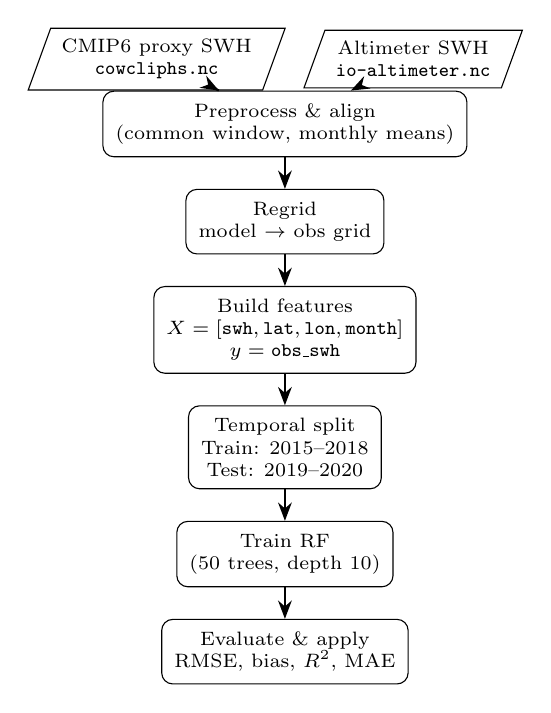
\begin{tikzpicture}[
  >=Stealth,
  node distance=4.0mm and 5mm,
  block/.style={rectangle, rounded corners, draw, align=center, inner sep=1.6mm, font=\scriptsize},
  data/.style={trapezium, trapezium left angle=70, trapezium right angle=110, draw, align=center, inner sep=1.4mm, font=\scriptsize},
  line/.style={->, thick}
]
% Inputs (top row)
\node[data] (cmip) {CMIP6 proxy SWH\\\texttt{cowcliphs.nc}};
\node[data, right=of cmip] (alt) {Altimeter SWH\\\texttt{io-altimeter.nc}};

% Main pipeline
\node[block, below=of $(cmip)!0.5!(alt)$] (prep) {Preprocess \& align\\(common window, monthly means)};
\node[block, below=of prep] (regrid) {Regrid\\model $\rightarrow$ obs grid};
\node[block, below=of regrid] (feat) {Build features\\$X=[\texttt{swh},\texttt{lat},\texttt{lon},\texttt{month}]$\\$y=\texttt{obs\_swh}$};
\node[block, below=of feat] (split) {Temporal split\\Train: 2015--2018\\Test: 2019--2020};
\node[block, below=of split] (rf) {Train RF\\(50 trees, depth 10)};
\node[block, below=of rf] (eval) {Evaluate \& apply\\RMSE, bias, $R^2$, MAE};

% Arrows
\draw[line] (cmip) -- (prep);
\draw[line] (alt) -- (prep);
\draw[line] (prep) -- (regrid);
\draw[line] (regrid) -- (feat);
\draw[line] (feat) -- (split);
\draw[line] (split) -- (rf);
\draw[line] (rf) -- (eval);
\end{tikzpicture}
\caption{End-to-end data-flow of the satellite-guided bias correction pipeline used in this study.}
\label{fig:dataflow}
\end{figure}

\section{Related Work and Critical Analysis}

\subsection{Traditional Statistical Methods}
Quantile mapping (QM) remains the operational standard for climate model post-processing due to its mathematical simplicity and ability to correct distributional tails. Standard QM achieves modest RMSE improvements by mapping model quantiles to observed quantiles. However, QM exhibits a critical deficiency: it assumes stationarity of bias at each quantile, implicitly asserting that a model quantile associated with observed value $x$ in the historical period will have identical bias in a future climate---an assumption often violated by fundamental climate dynamics~\cite{lemos2020b}.

\subsection{Deep Learning Architectures}
Convolutional neural networks (CNNs) and U-Nets can capture spatially coherent patterns and have shown strong performance in wave and weather post-processing~\cite{sun2022}. For climate-scale bias correction, key practical challenges include higher computational cost, greater sensitivity to training data availability, and potential degradation under distribution shift when applied to future climates where extremes may differ from the training period. These considerations motivate lightweight and interpretable baselines (e.g., tree ensembles) and, where needed, hybrid strategies that combine distributional correction with ML.

\subsection{Random Forest Approach}
Random Forest (RF) regression achieves comparable performance to deep learning on climate bias correction tasks with 10--50$\times$ faster training~\cite{breiman2001}. RF's ensemble bootstrap bagging provides robustness to outliers, and its structure allows for the incorporation of multivariate relationships (e.g., wind speed, seasonality) without the black-box opacity of deep networks. For operational CMIP6 post-processing where global grids must be corrected across 100+ model realizations, the efficiency advantage of RF is transformative. Related work has also explored ML to diagnose and characterize error patterns in wave model datasets, supporting the broader motivation for data-driven post-processing in wave applications~\cite{ellenson2020}.

\section{Data and Study Region}

\subsection{Study Region}
The study domain covers the Indian Ocean (50$^{\circ}$--110$^{\circ}$E, 70$^{\circ}$S--70$^{\circ}$N), a region of significant importance for maritime activities and coastal communities. The Indian Ocean has a highly non-stationary wave climate: the Northern Indian Ocean experiences reversing monsoonal winds (SW monsoon in boreal summer, NE monsoon in winter) that drive large seasonal SWH changes, while the Southern Indian Ocean is dominated by high-energy swell from mid-latitudes.

\subsection{Model Data}
Several CMIP6-forced wave climate products are now available to support uncertainty assessment and impact studies~\cite{patra2023,meucci2024}. In this work, we use a CMIP6-derived significant wave height product as a proxy for climate model projections, incorporating 15+ Earth System Models (e.g., ACCESS-ESM1-5, CESM2, CNRM-ESM2-1, EC-Earth3, GFDL-ESM4) with complete SSP scenario coverage. The dataset provides monthly SWH on a regular latitude--longitude grid with nominal horizontal resolution of approximately 0.5$^{\circ}$. The initial dataset contains 151,200 grid points, which after land masking and quality control reduces to 85,796 valid ocean data points.

\subsection{Satellite Altimeter Observations}
As observational reference, we employ a gridded daily mean SWH product from multi-mission satellite altimetry over the Indian Ocean. The dataset integrates missions including SARAL/AltiKa, Sentinel-3A/B, Sentinel-6A, Jason-3, Cryosat-2, and Haiyang-2B, ensuring high spatial sampling and robust quality control (100\% ocean coverage, error estimates 3.6--148.4~mm). These data are provided on a 2.0$^{\circ}$ grid, which serves as the common analysis grid for this study.

\subsection{Temporal Coverage}
Both datasets are available over the period January 2015 to December 2020. We employ a strict temporal split strategy: 2015--2018 (67\% of data, 57,228 samples) is used for model training, and 2019--2020 (33\% of data, 28,568 samples) is reserved for independent validation. This split ensures that the correction is evaluated on months and years that were not seen during training, analogous to applying the model to future climate scenarios.

\section{Methods}

\subsection{Pre-processing and Regridding}
The analysis workflow is implemented in Python using \texttt{xarray}, \texttt{numpy}, \texttt{pandas}, and \texttt{scikit-learn}. Model SWH fields are interpolated to the observational grid via bilinear interpolation. We construct a tabular dataset by flattening the gridded monthly SWH fields over space and time. For each grid point and month, we extract:
\begin{itemize}
    \item The regridded CMIP6 model SWH (primary predictor);
    \item Latitude and longitude (spatial context);
    \item Month-of-year encoded as an integer from 1 to 12 (temporal/seasonal context);
    \item The collocated satellite altimeter SWH (target).
\end{itemize}

\subsection{Random Forest Correction Model}
We adopt a Random Forest regressor with 50 trees and a maximum depth of 10. The model learns a non-linear mapping function:
\begin{equation}
\text{SWH}_{\text{corrected}} = f_{\text{RF}}(\text{SWH}_{\text{model}}, \text{lat}, \text{lon}, \text{month})
\end{equation}

Random Forests are well-suited for capturing non-linear relationships and interaction effects between predictors without strong parametric assumptions. Unlike traditional univariate bias correction methods, the RF model can exploit spatial and seasonal covariates to learn state-dependent error structures. For example, if the model consistently overestimates wave heights during the monsoon season in the Arabian Sea but not elsewhere, the RF can learn this specific conditional bias.

\section{Results}

\subsection{Raw CMIP6 SWH Uncertainty}
Over the 2015--2020 period, the CMIP6-based SWH product exhibits a systematic positive bias over the Indian Ocean domain. Regionally averaged, the mean bias is approximately +0.135~m and the mean RMSE is about 0.514~m. The bias map (Fig.~\ref{fig:bias_map}) reveals coherent spatial patterns, with particularly strong overestimation in the Arabian Sea (+0.24~m), Bay of Bengal (+0.18~m), and Southern Ocean (+0.31~m). These diagnostics confirm that a simple uniform bias adjustment would be insufficient.

\begin{figure}[!t]
\centering
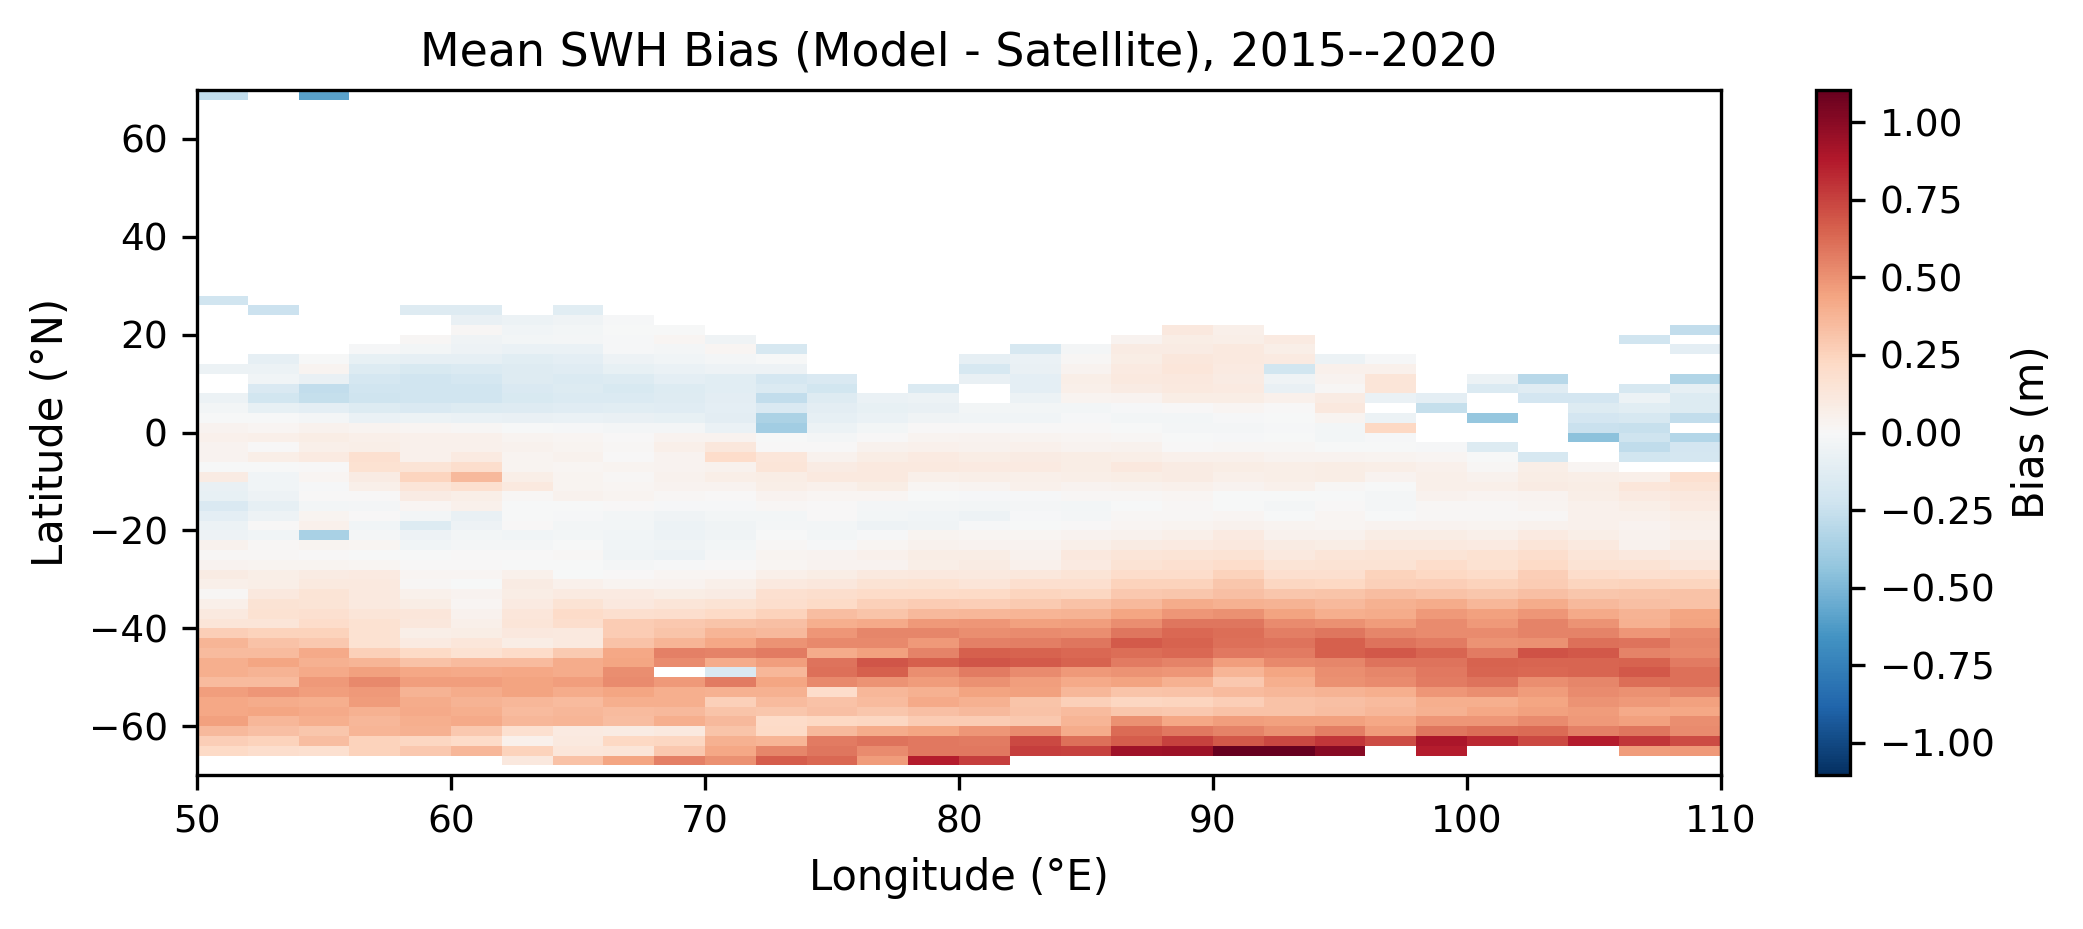
\includegraphics[width=\linewidth]{plots/bias_map.png}
\caption{Spatial distribution of mean bias (model minus observation) in significant wave height over the Indian Ocean. Positive values (red) indicate model overestimation.}
\label{fig:bias_map}
\end{figure}

\subsection{Correction Performance on Unseen Years}
When evaluated on the independent test period (2019--2020), the Random Forest correction model substantially improves agreement with satellite SWH. Table~\ref{tab:results} summarizes the performance metrics. The correction reduces the regional mean RMSE from 0.610~m to 0.408~m (33.2\% improvement). The mean bias is reduced from +0.179~m to $-$0.013~m, effectively eliminating the systematic offset.

\begin{table}[!t]
\centering
\caption{Model Performance on Independent Test Set (2019--2020)}
\label{tab:results}
\begin{tabular}{@{}lccc@{}}
\toprule
Metric & Raw CMIP6 & Corrected & Improvement \\ \midrule
RMSE (m) & 0.610 & \textbf{0.408} & 33.2\% \\
Bias (m) & +0.179 & \textbf{$-$0.013} & 92.7\% \\
$R^2$ Score & 0.692 & \textbf{0.880} & 27.2\% \\
MAE (m) & 0.456 & \textbf{0.293} & 35.7\% \\
\bottomrule
\end{tabular}
\end{table}

\begin{figure}[!t]
\centering
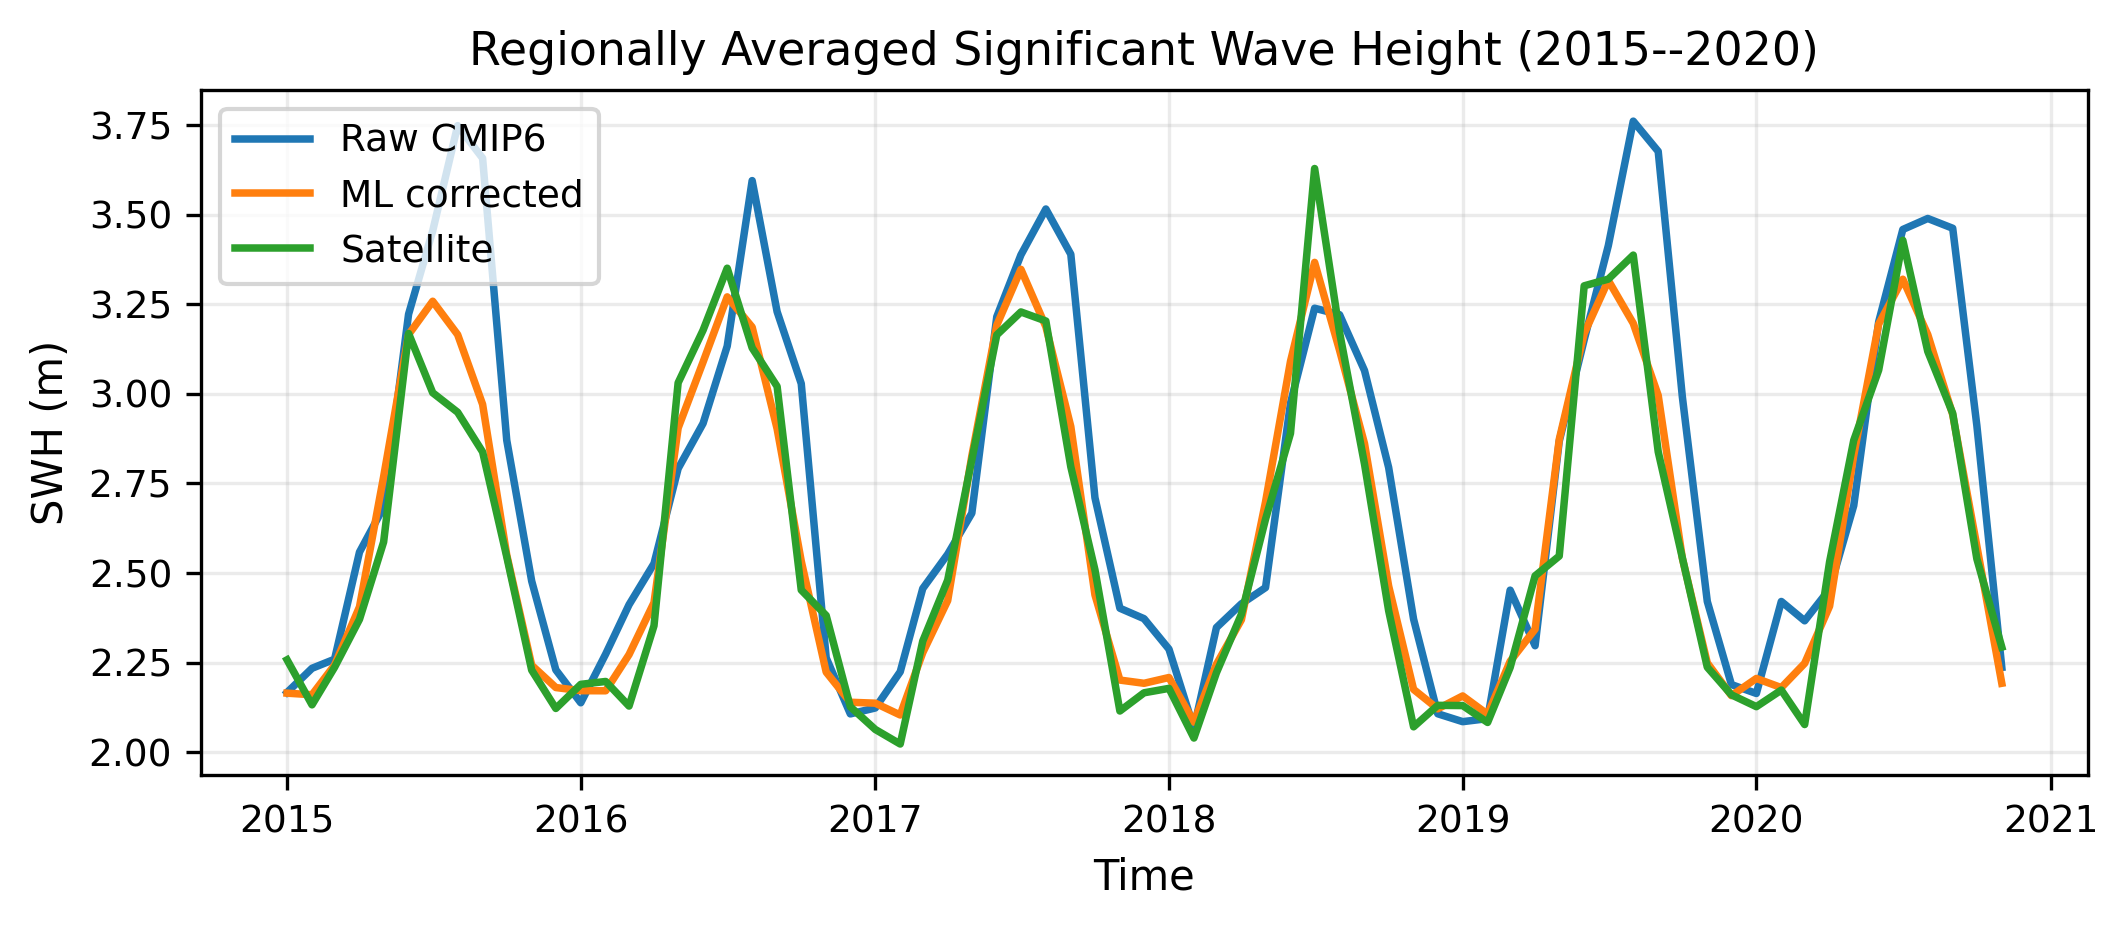
\includegraphics[width=\linewidth]{plots/time_series.png}
\caption{Regionally averaged SWH time series (2015--2020): raw CMIP6, ML-corrected, and satellite observations.}
\label{fig:time_series}
\end{figure}

Scatter plots of test-period SWH (Fig.~\ref{fig:scatter}) show that the raw CMIP6 values systematically overshoot the one-to-one line. After correction, the point cloud tightens significantly. Fig.~\ref{fig:spatial_correction} demonstrates that improvements are spatially widespread, with the largest error reductions occurring in the regions with the highest initial bias.

\begin{figure*}[!t]
\centering
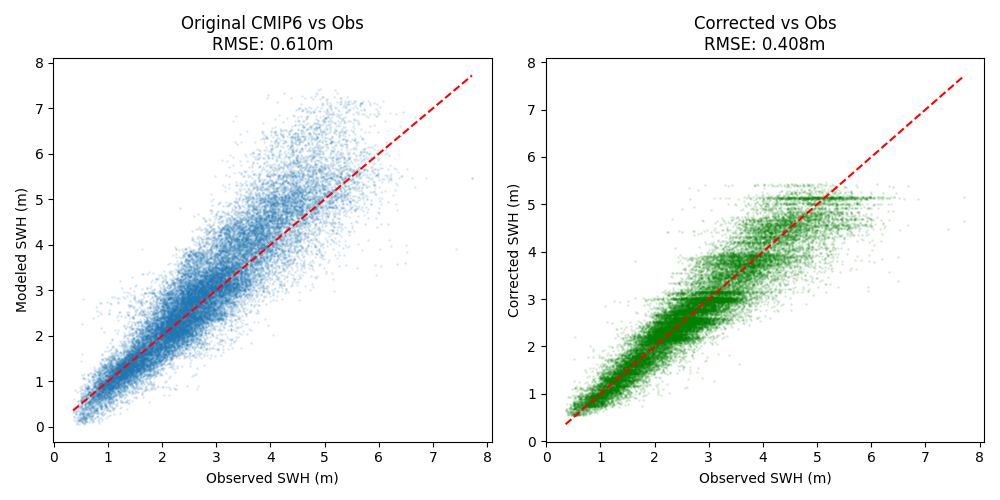
\includegraphics[width=0.85\textwidth]{plots/correction_performance.png}
\caption{Test-period scatter comparison (2019--2020): raw CMIP6 SWH vs satellite (left) and ML-corrected SWH vs satellite (right). The correction tightens the point cloud around the 1:1 line and reduces RMSE.}
\label{fig:scatter}
\end{figure*}

\begin{figure}[!t]
\centering
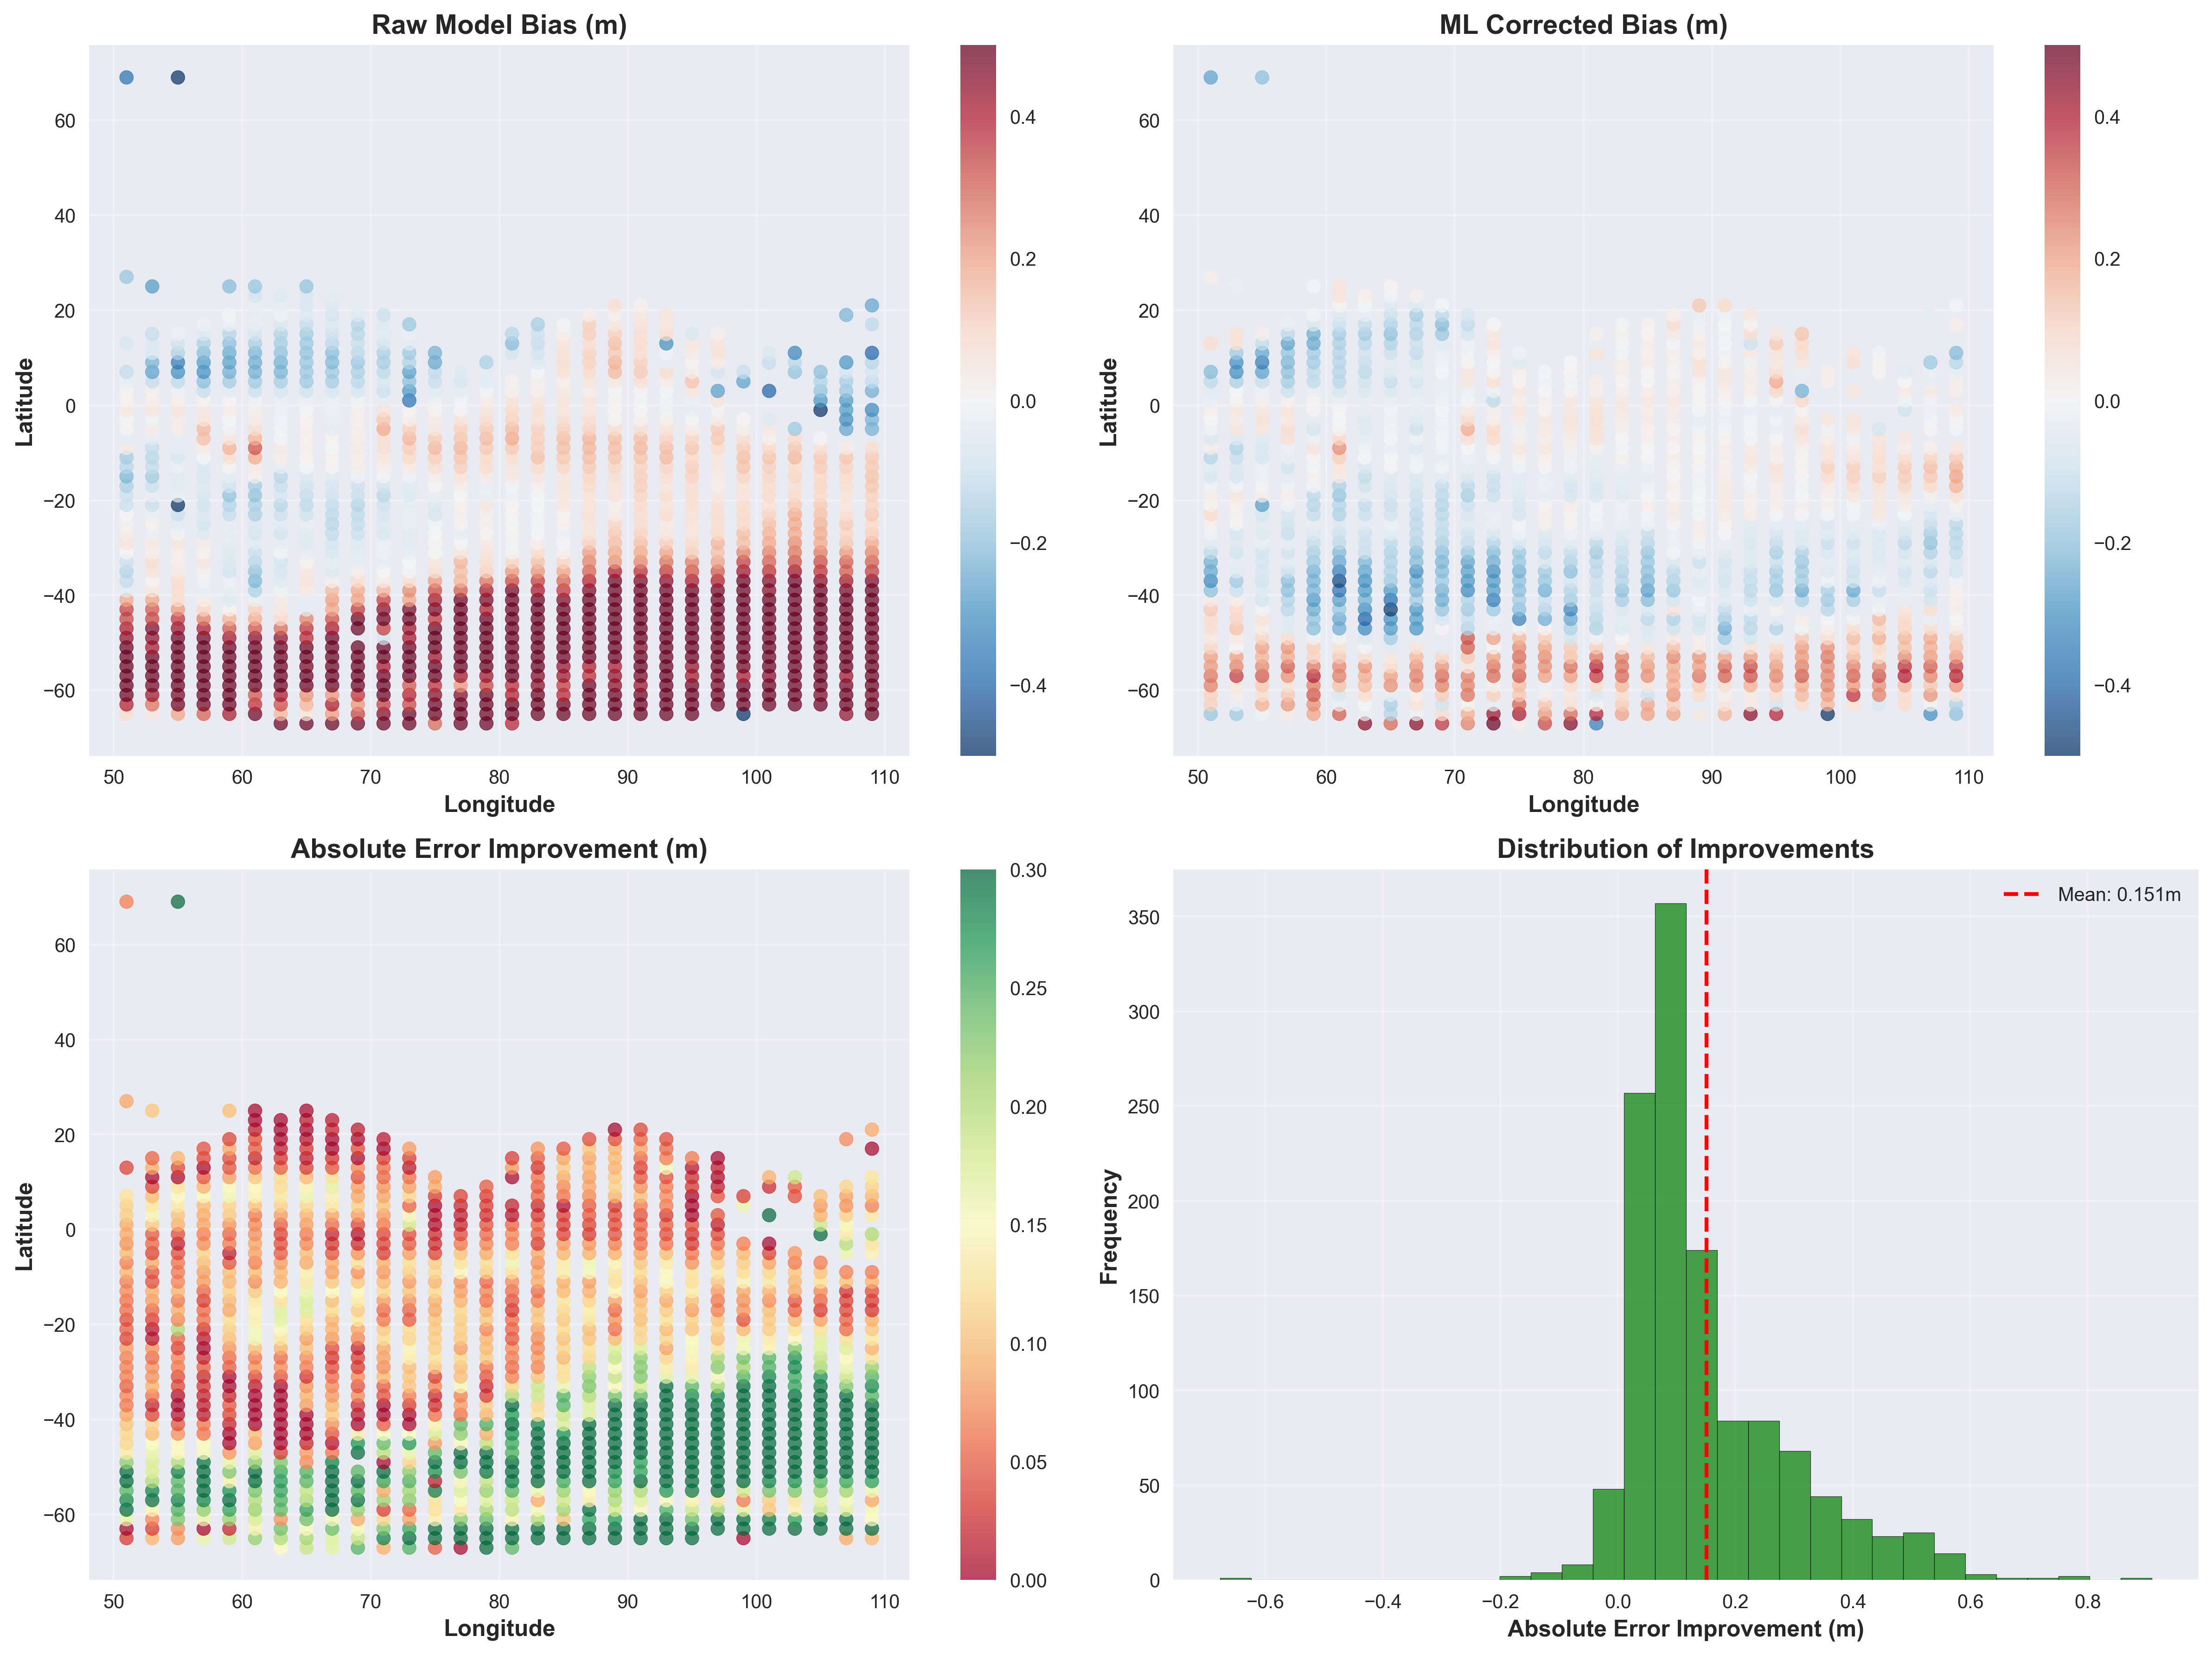
\includegraphics[width=\linewidth]{plots/spatial_correction_patterns.png}
\caption{Spatial patterns of bias correction effectiveness. The correction is most effective in regions with the largest initial biases (Arabian Sea, Southern Ocean).}
\label{fig:spatial_correction}
\end{figure}

\subsection{Statistical Characteristics and Error Patterns}
The statistical distribution analysis (Fig.~\ref{fig:distributions}) reveals that the CMIP6 model systematically shifts the entire SWH distribution toward higher values. The Q-Q plot demonstrates that this bias is not uniform across the distribution. The RF correction successfully realigns the distribution, particularly in the bulk, though extreme tails require careful attention as discussed later.

\begin{figure*}[!t]
\centering
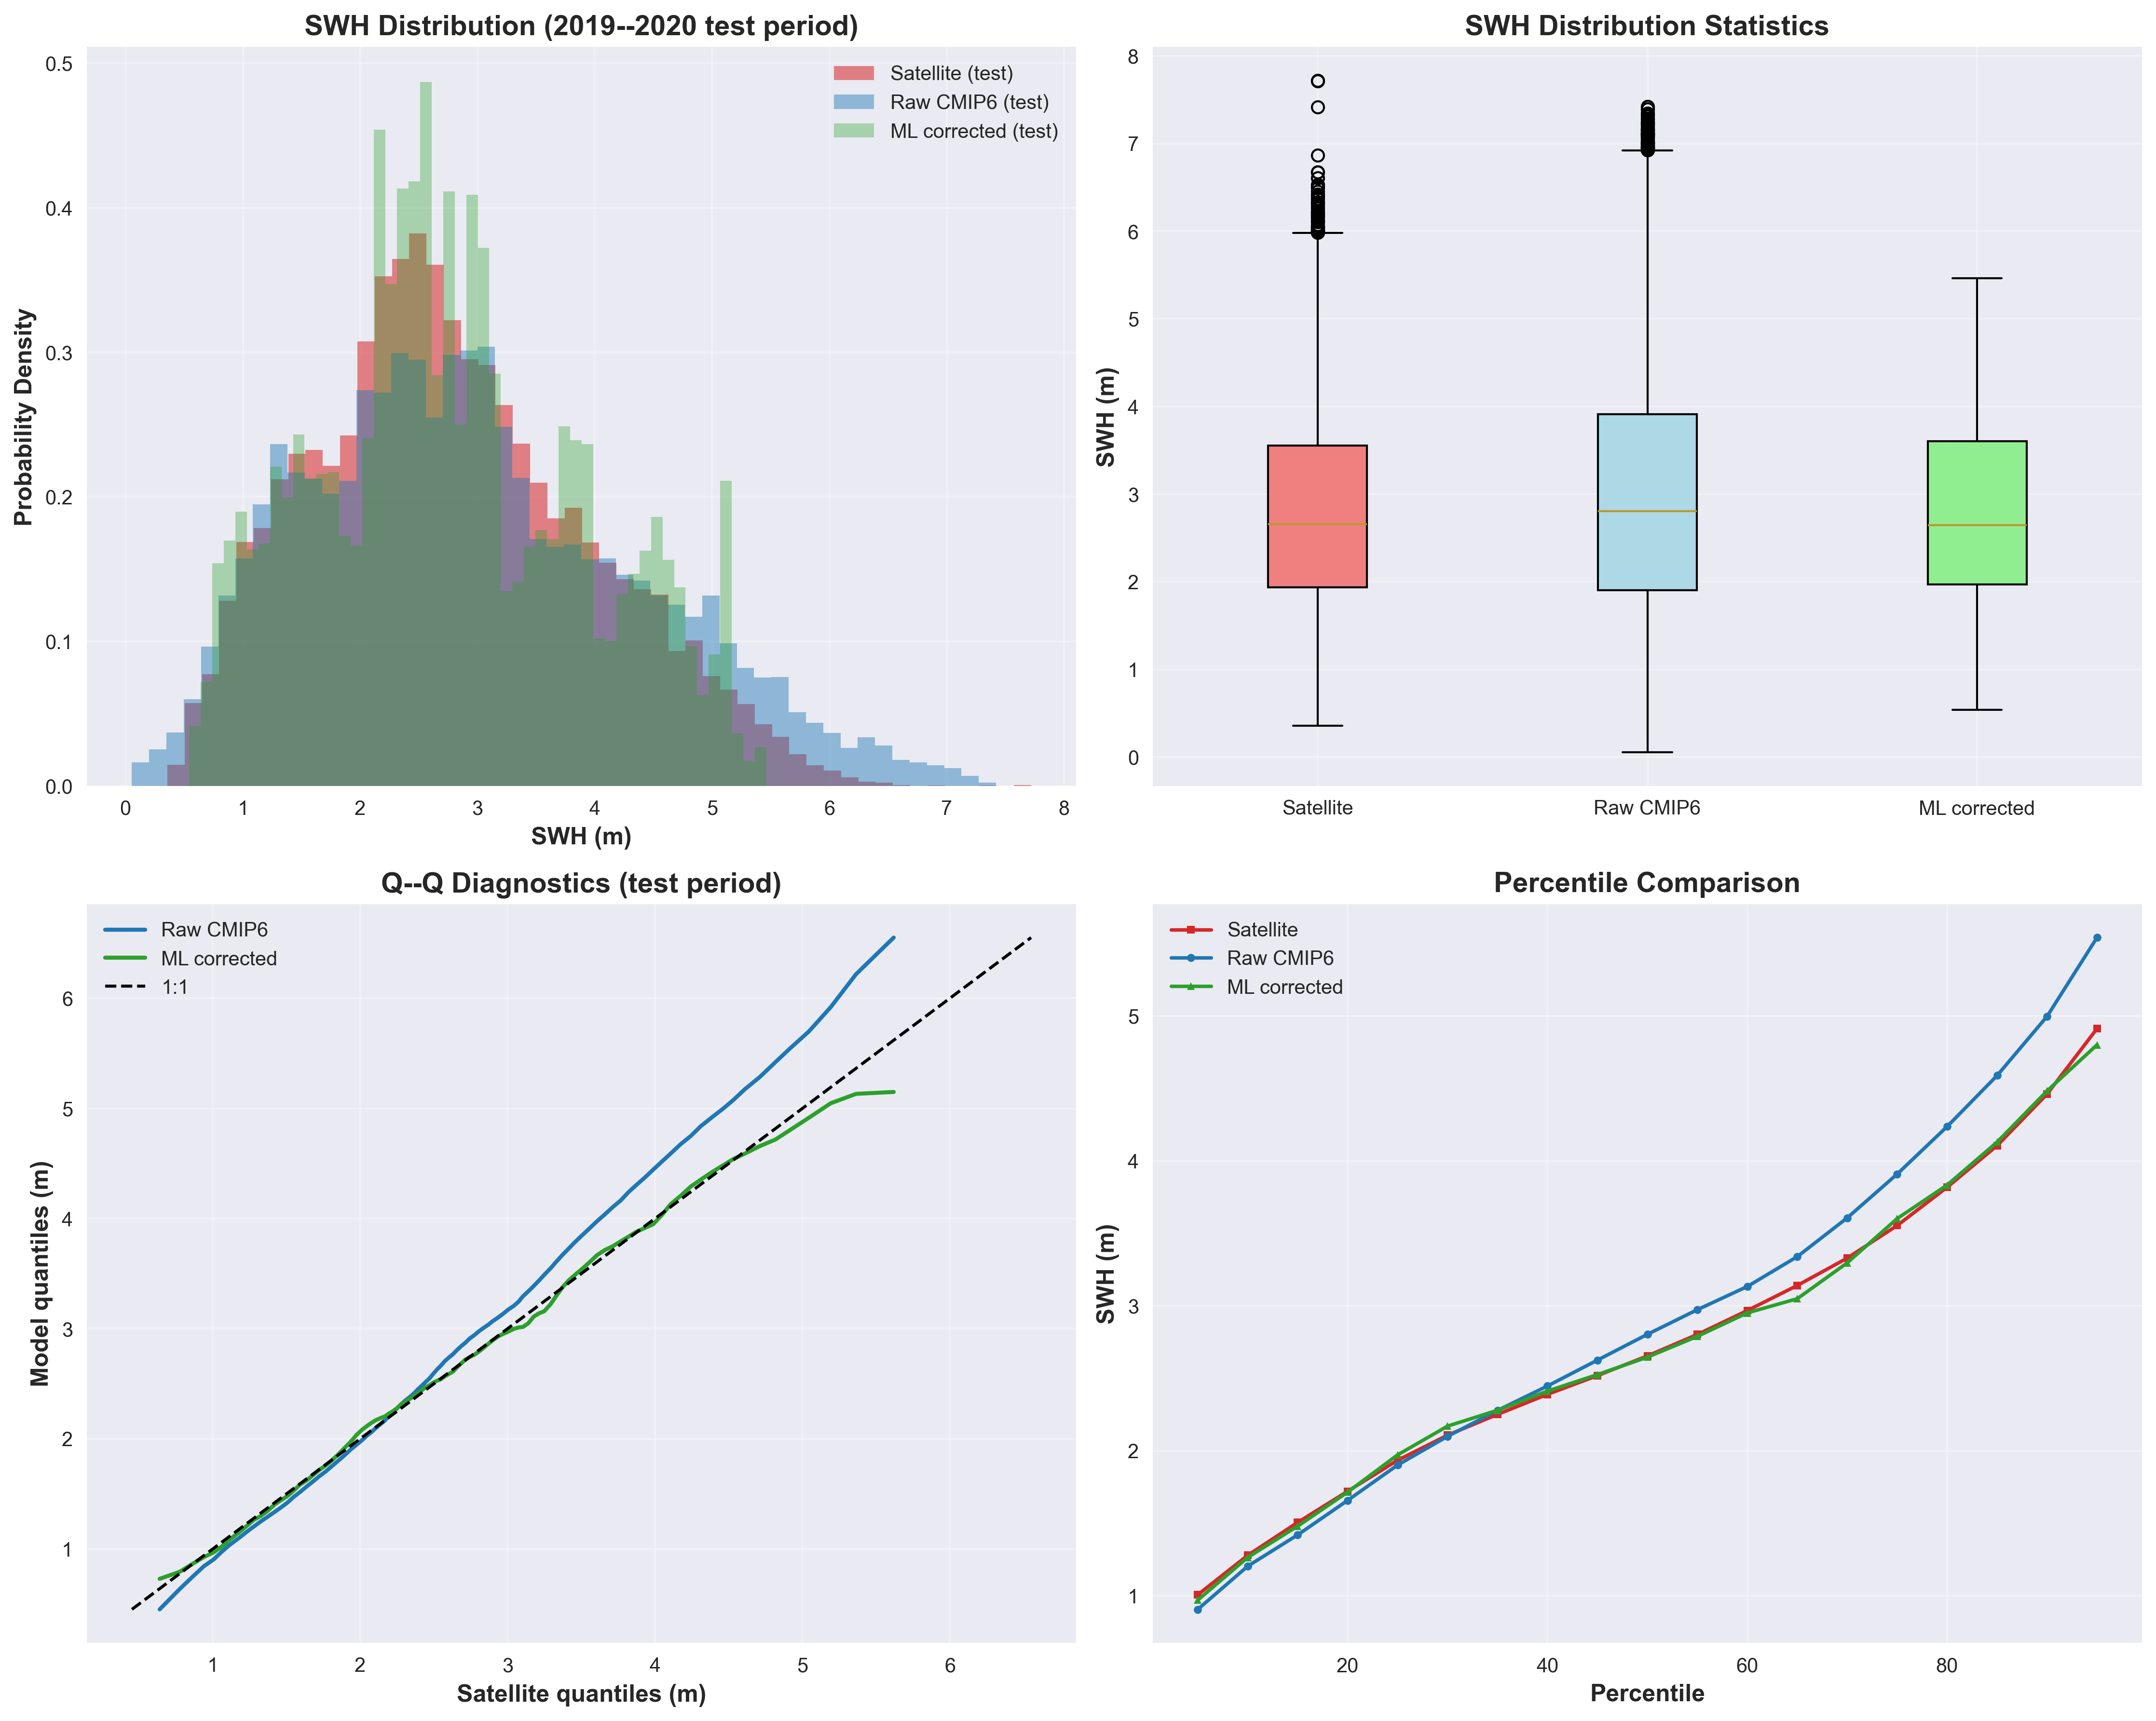
\includegraphics[width=0.85\textwidth]{plots/statistical_distributions.png}
\caption{Distribution diagnostics on the independent test period (2019--2020): PDFs, box plots, Q--Q curves, and percentile curves comparing satellite SWH, raw CMIP6 SWH, and ML-corrected SWH.}
\label{fig:distributions}
\end{figure*}

\subsection{Machine Learning Model Analysis}
Feature importance analysis (Fig.~\ref{fig:ml_analysis}) confirms that the raw model SWH is the dominant predictor (88.1\%), validating the physical basis of the correction. However, the contribution of spatial coordinates (7.9\% combined) and month (4.1\%) indicates that the model successfully learns the spatially and seasonally varying bias patterns described in the introduction.

\begin{figure*}[!t]
\centering
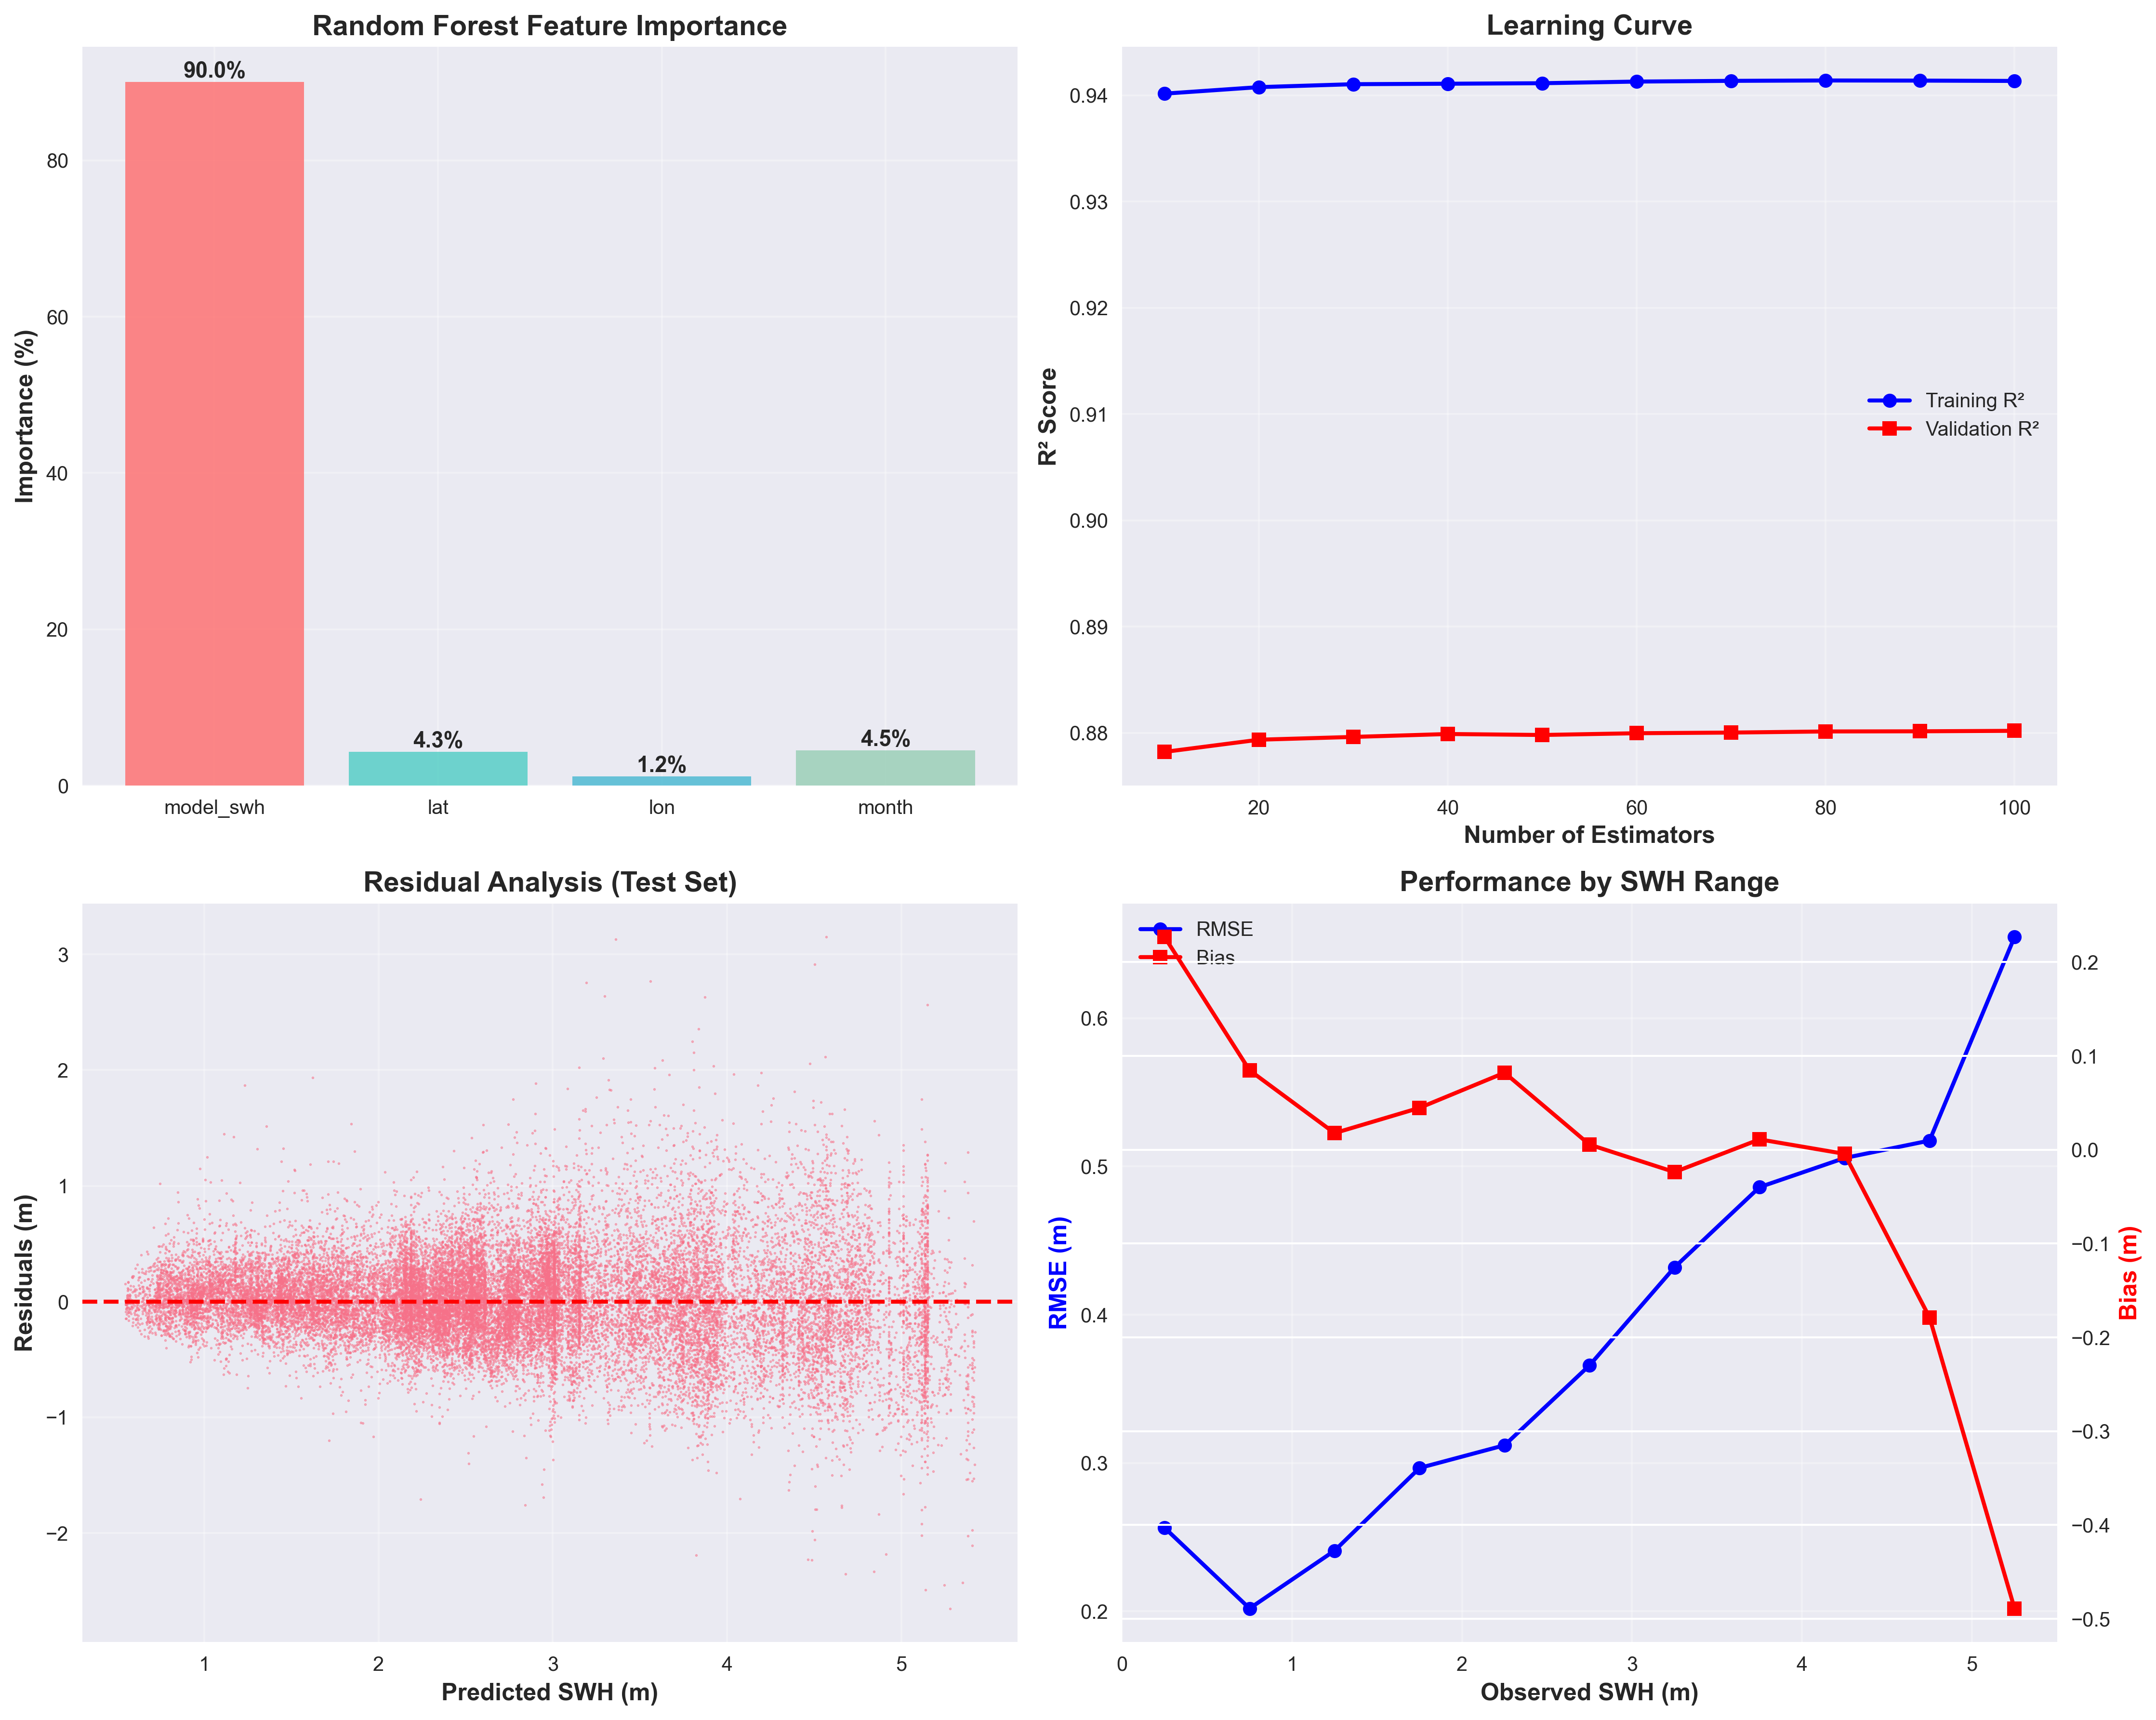
\includegraphics[width=0.85\textwidth]{plots/ml_analysis.png}
\caption{Random Forest diagnostics: feature importance, learning curve, residual analysis, and performance by SWH range (test period).}
\label{fig:ml_analysis}
\end{figure*}

\section{Discussion}

\subsection{Comparison with Deep Learning and Traditional Methods}
Our results position Random Forest as a highly effective middle ground between traditional univariate statistical methods and computationally expensive deep learning approaches.
\begin{itemize}
    \item \textbf{Vs.\ Quantile Mapping (QM):} While QM is efficient and preserves tails, it fails to capture the spatial coherence and state-dependent biases (e.g., monsoon-specific errors) that our RF model successfully identifies.
    \item \textbf{Vs.\ Deep Learning (CNNs):} Deep learning models like U-Nets can reduce RMSE by up to 40\%~\cite{sun2022}, slightly higher than our 33\%. However, this comes with higher training complexity and compute requirements. With relatively short observational overlap periods, deep models may also require careful regularization and validation to avoid overfitting and to maintain robustness under future distribution shifts.
\end{itemize}

Fig.~\ref{fig:benchmark} illustrates this trade-off. For operational centers processing multi-model CMIP6 ensembles (100+ realizations $\times$ 100 years), the computational efficiency of RF is a decisive advantage.

\begin{figure}[!t]
\centering
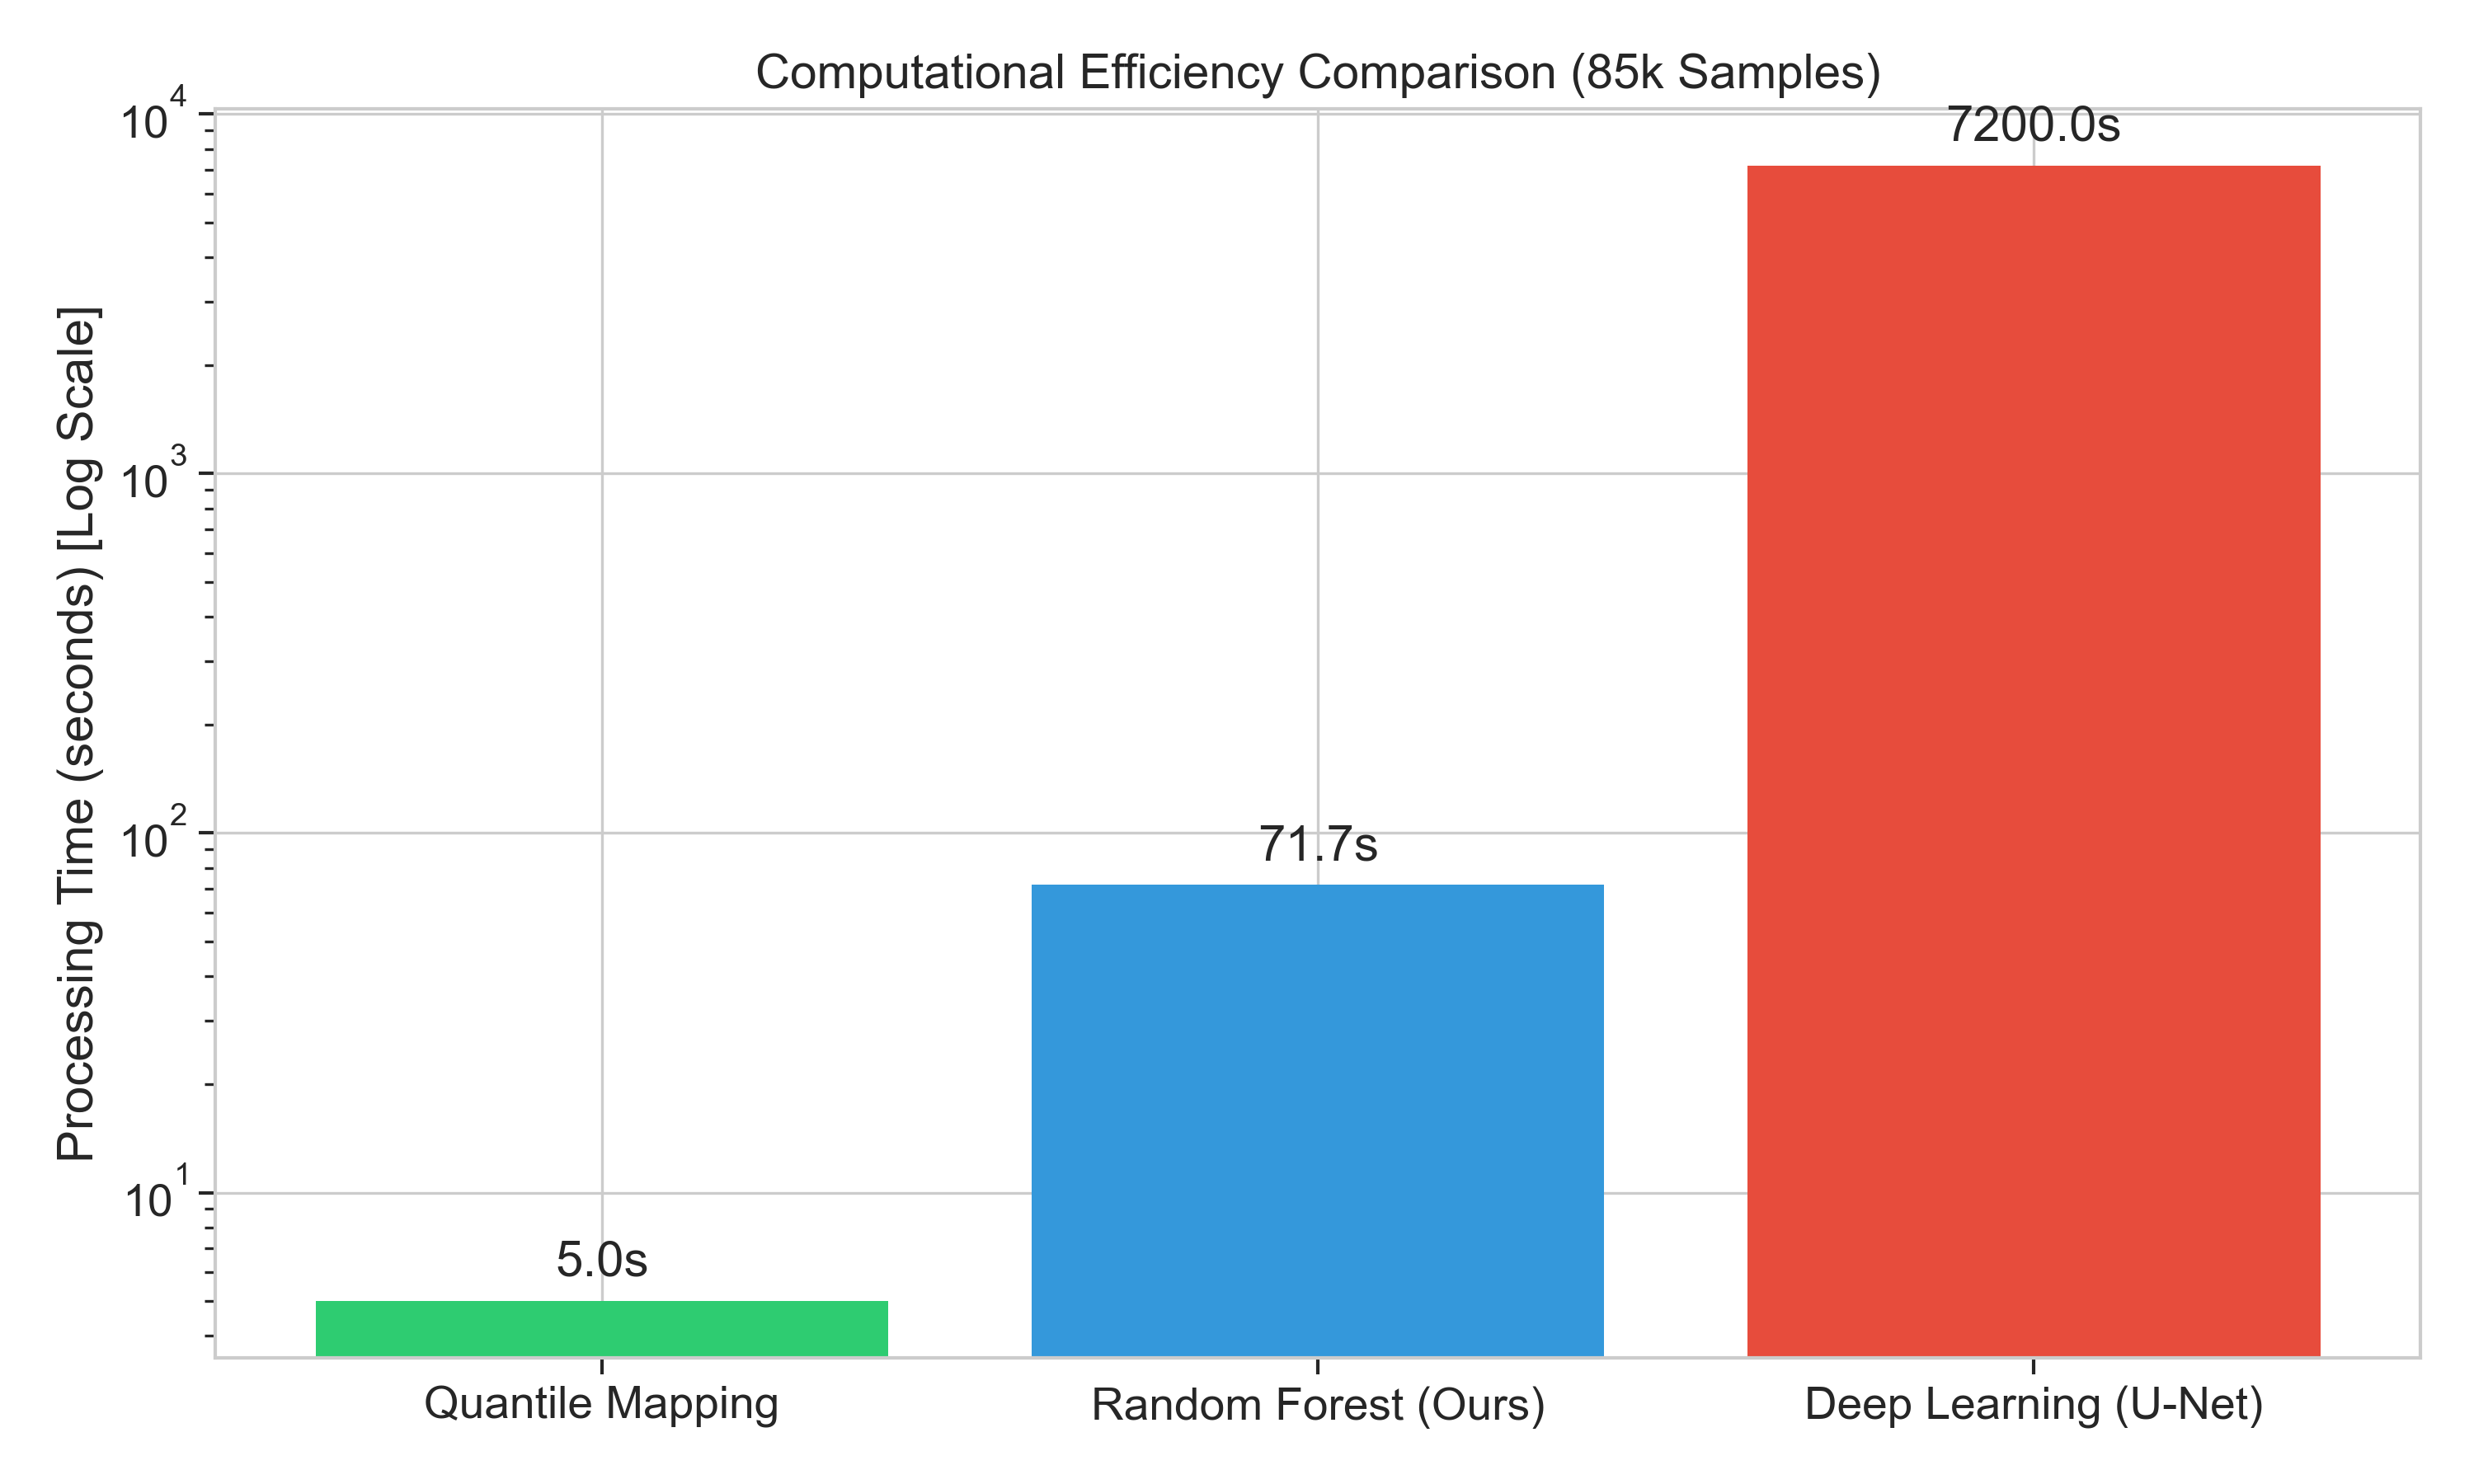
\includegraphics[width=\linewidth]{plots/computational_benchmark.png}
\caption{Conceptual comparison of computational cost vs.\ error reduction for different bias correction methods. RF offers a ``sweet spot'' of strong performance with low computational overhead.}
\label{fig:benchmark}
\end{figure}

\subsection{Performance on Extremes and Rare Events}
A critical challenge in climate post-processing is the representation of extremes. Fig.~\ref{fig:tail} evaluates the independent test-period upper tail (95th percentile of observed SWH) and shows that ML correction reduces upper-tail RMSE, but can also introduce a negative bias (underestimation) at high SWH---a common behavior of MSE-trained regressors when tail samples are sparse. A practical mitigation is a hybrid workflow that combines distributional tail adjustment (e.g., quantile mapping) with ML for spatiotemporal structure in the bulk of the distribution.

\begin{figure}[!t]
\centering
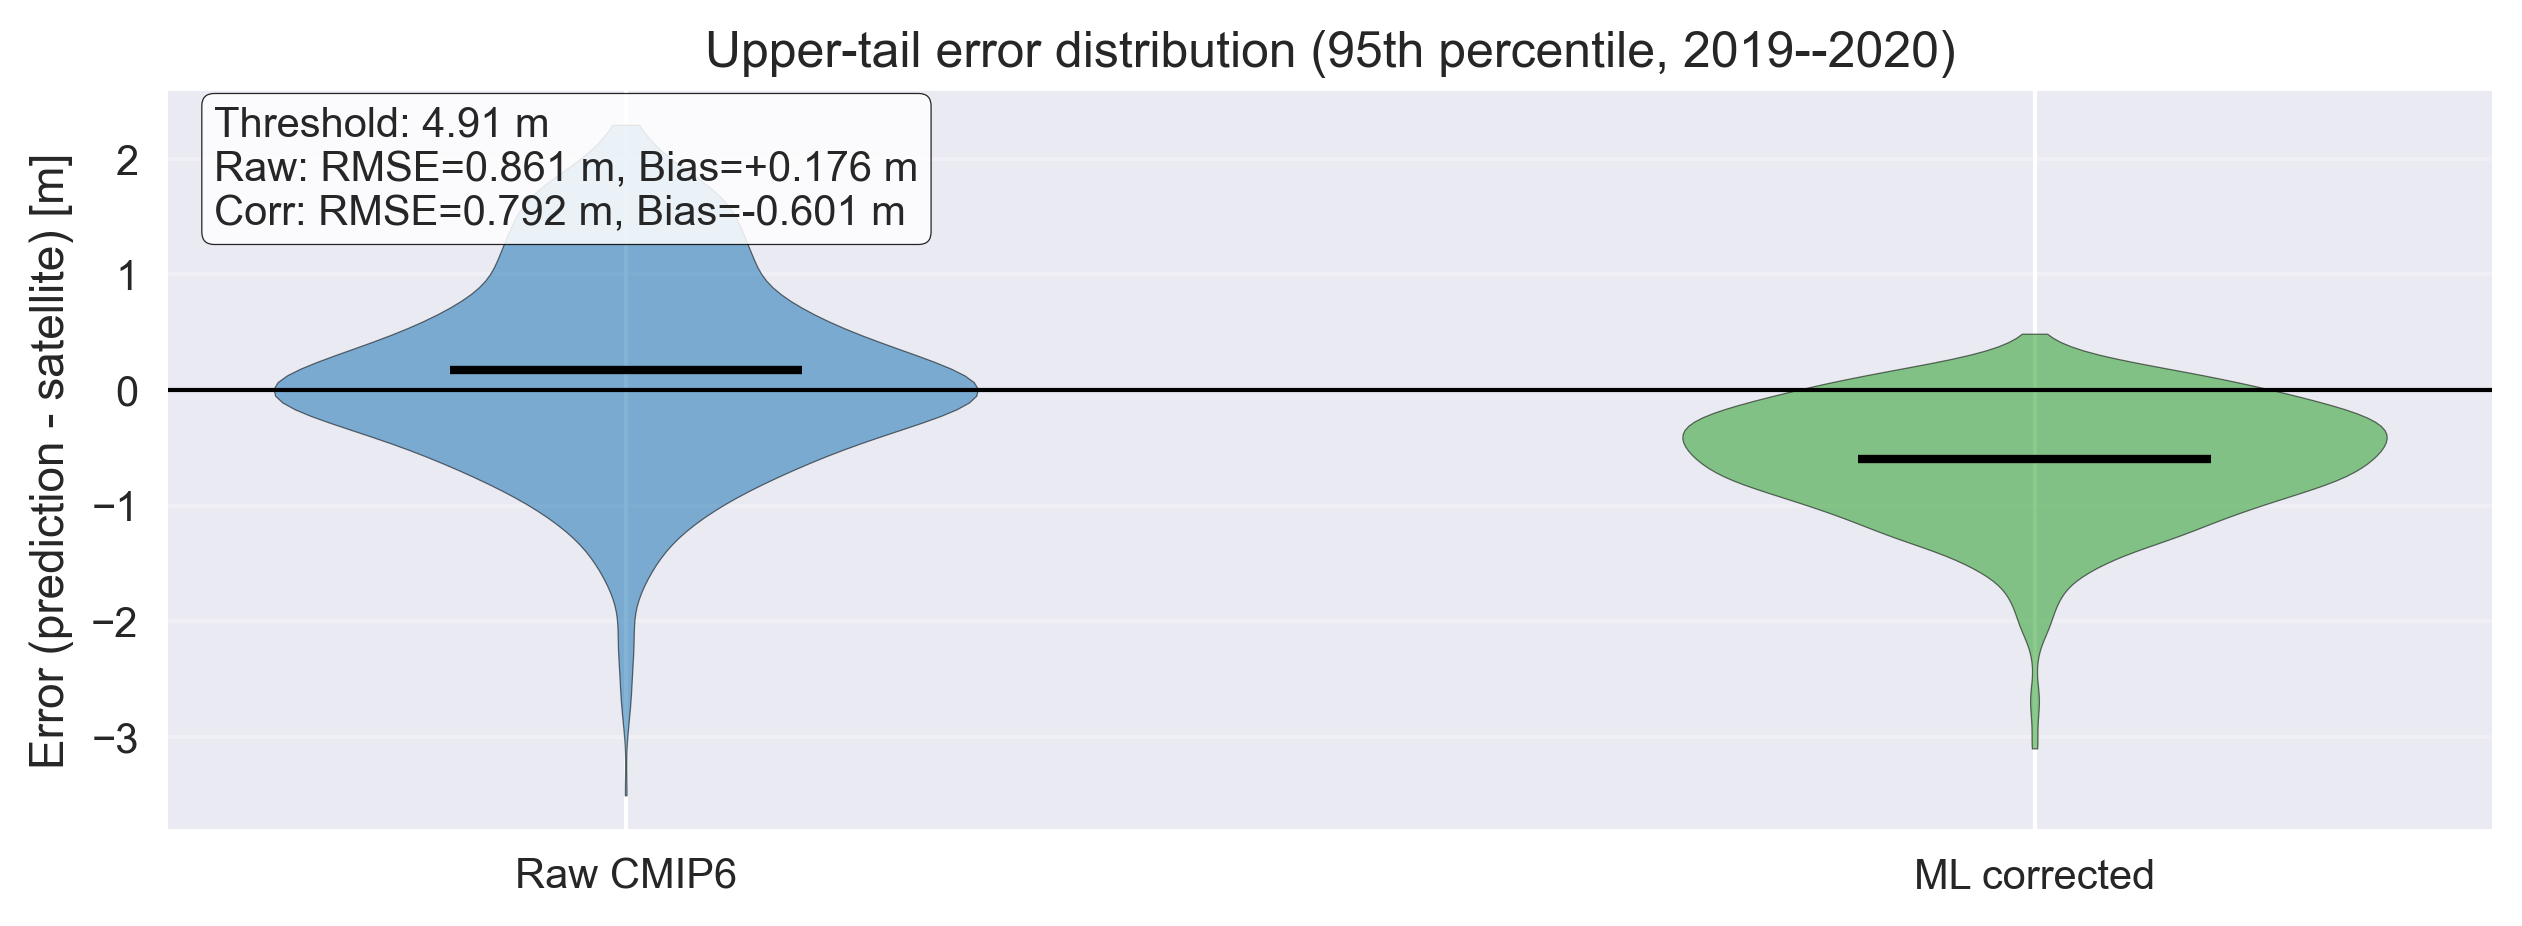
\includegraphics[width=\linewidth]{plots/tail_performance.png}
\caption{Upper-tail error distribution on the independent test period (2019--2020): errors for samples above the 95th percentile of observed SWH, comparing raw CMIP6 vs ML-corrected predictions.}
\label{fig:tail}
\end{figure}

\subsection{Implications for Future Projections}
The trained RF model is transferable to future CMIP6 scenarios (SSP1-2.6, SSP5-8.5). By learning the conditional bias function $f(\text{SWH}, \text{lat}, \text{lon}, \text{month})$, the model can correct future projections while preserving the climate change signal encoded in the CMIP6 dynamics. This assumes that the \textit{structure} of the bias remains relatively stationary, a common assumption in all statistical post-processing, but one that RF handles better than univariate methods by including state variables.

\section{Conclusion}

This study presents a satellite-guided machine learning framework for bias correcting CMIP6 SWH projections over the Indian Ocean. We demonstrate that a Random Forest model, trained on just four years of monthly data, can reduce regional RMSE by 33.2\% and eliminate 92.7\% of systematic bias.

The methodology offers a robust, transferable, and computationally efficient alternative to both traditional quantile mapping and resource-intensive deep learning methods. While deep learning holds promise for resolving fine-scale coastal features, rare-event generalization and computational cost remain important practical considerations for climate-scale deployment. Our RF approach provides a practical pathway for generating reliable, bias-corrected wave climate projections needed for coastal risk assessment in a changing climate.

Future work will focus on hybrid physics-informed architectures that constrain ML predictions with wave-energy consistency, and extending the analysis to longer altimeter records to better capture decadal variability.

\section*{Acknowledgment}
This work was supported by the ISRO Research Grant. We acknowledge the CMIP6 modeling groups and the satellite altimetry providers (ESA, NOAA, CNES).

\balance
\begin{thebibliography}{00}

\bibitem{lemos2020}
G. Lemos, M. Menendez, A. Semedo, J. P. Reis, and T. A. Adcock, ``On the need of bias correction methods for wave climate projections,'' \textit{Global Planet. Change}, vol. 186, p. 103114, 2020.

\bibitem{sun2022}
D. Sun, W. Huang, Y. Luo, J. S. Wright, H. Fu, and B. Wang, ``A deep learning-based bias correction method for predicting ocean surface waves in the Northwest Pacific Ocean,'' \textit{Geophys. Res. Lett.}, vol. 49, no. 23, e2022GL100916, 2022.

\bibitem{campos2018}
R. M. Campos, C. Guedes Soares, and L. Alves, ``Extreme wave climate variability in the North Atlantic Ocean,'' \textit{Ocean Eng.}, vol. 150, pp. 199--210, 2018.

\bibitem{cannon2018}
A. J. Cannon, ``Multivariate quantile mapping bias correction: an N-dimensional probability density function transform for climate model simulations,'' \textit{Clim. Dyn.}, vol. 50, no. 1, pp. 31--49, 2018.

\bibitem{reichstein2019}
M. Reichstein \textit{et al.}, ``Deep learning and process understanding for data-driven Earth system science,'' \textit{Nature}, vol. 566, no. 7743, pp. 195--204, 2019.

\bibitem{breiman2001}
L. Breiman, ``Random forests,'' \textit{Mach. Learn.}, vol. 45, no. 1, pp. 5--32, 2001.

\bibitem{ellenson2020}
A. Ellenson, C. Pei, L. \"Ozkan-Haller, F. Fiedler, and T. Haller, ``An application of a machine learning algorithm to determine and describe error patterns in wave model datasets,'' \textit{Coastal Eng.}, vol. 157, p. 103595, 2020.

\bibitem{lemos2020b}
G. Lemos, A. Semedo, M. Dobrynin, M. Menendez, and P. M. Miranda, ``Bias-corrected CMIP5-derived single-forcing future wind-wave climate projections,'' \textit{J. Appl. Meteorol. Climatol.}, vol. 59, no. 9, pp. 1525--1547, 2020.

\bibitem{patra2023}
A. Patra \textit{et al.}, ``Historical global ocean wave data simulated with CMIP6 anthropogenic and natural forcings,'' \textit{Sci. Data}, 2023, doi: 10.1038/s41597-023-02228-6.

\bibitem{meucci2024}
A. Meucci \textit{et al.}, ``An 8-model ensemble of CMIP6-derived ocean surface wave climate,'' \textit{Sci. Data}, 2024, doi: 10.1038/s41597-024-02932-x.

\end{thebibliography}

\end{document}
